\documentclass[12pt,a4paper]{article} 

\usepackage[spanish]{babel} 
\usepackage[utf8]{inputenc}
\usepackage[numbers,sort&compress]{natbib} 
\usepackage{graphicx} 
\usepackage{amsfonts}
\usepackage[left=2cm,right=2cm,top=2cm,bottom=2cm]{geometry}
\usepackage{listings}
\usepackage[usenames,dvipsnames]{color}
\lstset{ 
  language={R},
  basicstyle=\scriptsize\ttfamily,
  numbers=left,
  numberstyle=\tiny\color{Blue},
  stepnumber=1,
  numbersep={4pt},
  backgroundcolor=\color{white},
  showstringspaces=false,
  showtabs=false,
  frame=single,
  rulecolor=\color{black},
  tabsize=2,
  captionpos=b,
  breaklines=true,
  breakatwhitespace=false,        
  keywordstyle=\color{RoyalBlue},
  commentstyle=\color{YellowGreen},
  stringstyle=\color{ForestGreen}
}

\title{Matemáticas Computacionales \\ Práctica 3: Métodos de Bisección} 
\author{Brenda Esthela Martinez Martinez  1874537}

\begin{document}
\maketitle
\section{Introducci\'{o}n}\label{sec:intro}

En esta práctica 3 se implementa un método de Análisis Numérico para determinar los ceros de una función. En general, encontrar los ceros de una función en un número finito pasos casi nunca es posible. Para ello se utilizan métodos de aproximación. Estos métodos son iterativos iniciando con una aproximacón $ x_{0} $ o un intervalo $ [a, b] $, calculamos aproximaciones sucesivas $x _{1}, x_{2},..., x_{n} $ y se escoge $ x_{n} $ como aproximación del cero de la función cuando se cumpla un criterio de paro.

Los codigos utilizados se encuentran en \cite{repositorio} y la informacion se basa en \cite{METNUM}
\section{Función 1}\label{sec:FUN1}

Resultados: Cero de $ f$ en $[ -0.2 , 0.1 ]$ es approx: $ 3.814697e-07$ con error $<= 5.722046e-07 $

\begin{figure}
\centering
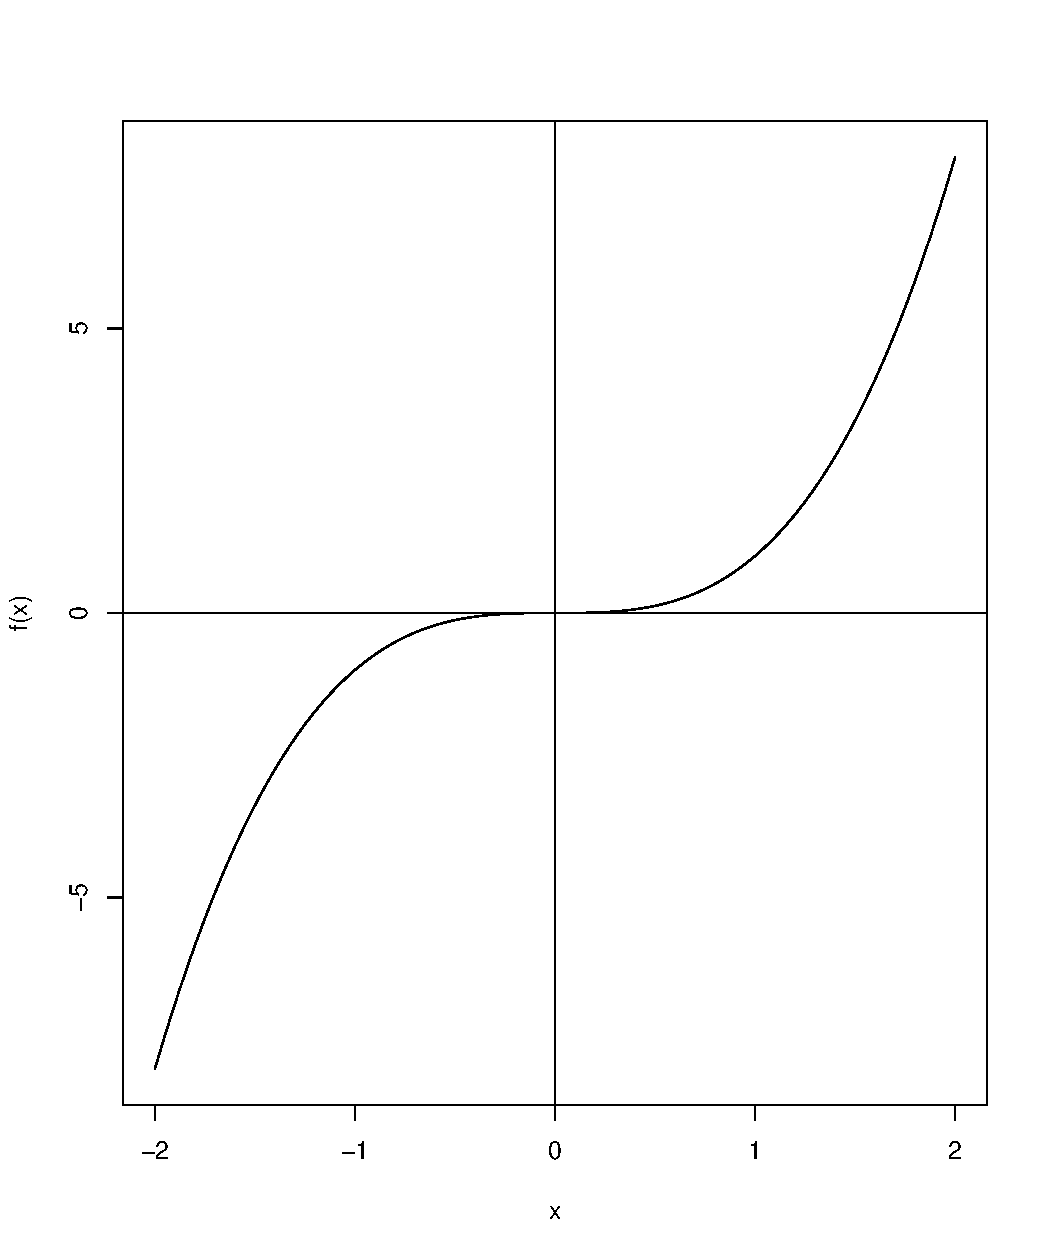
\includegraphics[scale=.8]{G1}
\caption{Grafica de la funcion 1}
\label{fig:G1}
\end{figure}

\begin{tabular}{| c | c | c | c |}
\hline
a & b & m & ERROR \\ \hline
-0.0500000   &    0.1000000   &   -0.0500000    &   0.0750000      \\
-0.0500000   &    0.0250000   &    0.0250000    &   0.0375000      \\
-0.0125000   &    0.0250000   &   -0.0125000    &   0.0187500      \\
-0.0125000   &    0.0062500   &    0.0062500    &   0.0093750      \\
-0.0031250   &    0.0062500   &   -0.0031250    &   0.0046875      \\
-0.0031250   &    0.0015625   &    0.0015625    &   0.0023437      \\
-0.0007812   &    0.0015625   &   -0.0007812    &   0.0011719      \\
-0.0007812   &    0.0003906   &    0.0003906    &   0.0005859      \\
-0.0001953   &    0.0003906   &   -0.0001953    &   0.0002930      \\
-0.0001953   &    0.0000977   &    0.0000977    &   0.0001465      \\
-0.0000488   &    0.0000977   &   -0.0000488    &   0.0000732      \\
-0.0000488   &    0.0000244   &    0.0000244    &   0.0000366      \\
-0.0000122   &    0.0000244   &   -0.0000122    &   0.0000183      \\
-0.0000122   &    0.0000061   &    0.0000061    &   0.0000092      \\
-0.0000031   &    0.0000061   &   -0.0000031    &   0.0000046      \\
-0.0000031   &    0.0000015   &    0.0000015    &   0.0000023      \\
-0.0000008   &    0.0000015   &   -0.0000008    &   0.0000011      \\
-0.0000008   &    0.0000004   &    0.0000004    &   0.0000006      \\ \hline
\end{tabular}
\newpage
\section{Función 2}\label{sec:FUN2}

Resultados:  Cero de $f$ en $[ 17 , 22.2 ]$ es approx:  $17.84636$ con error $<= 6.198883e-07 $

\begin{figure}
\centering
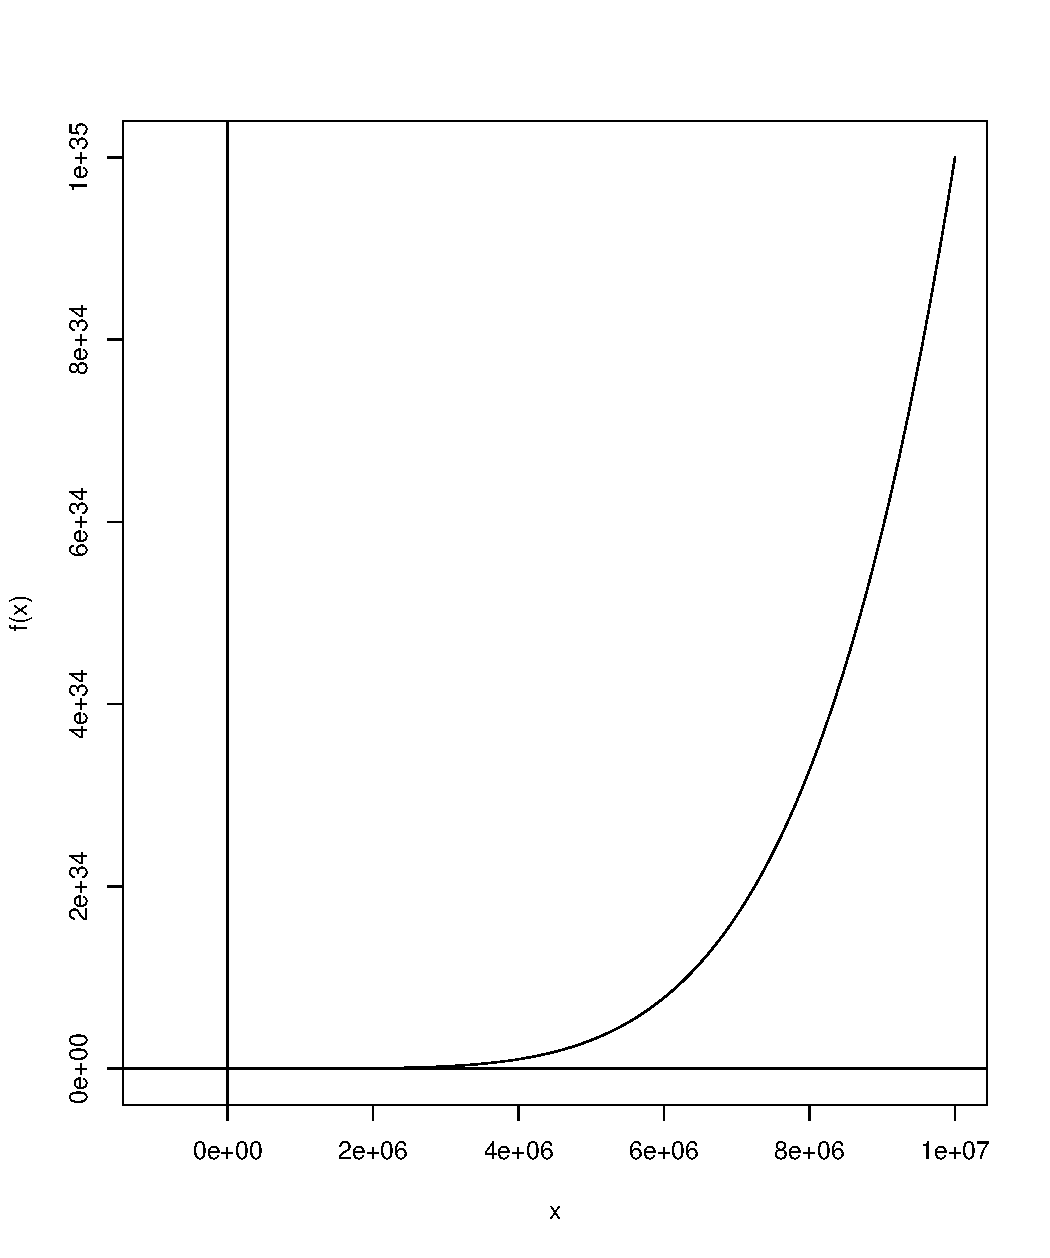
\includegraphics[scale=.8]{G2}
\caption{Grafica de la funcion 1}
\label{fig:G2}
\end{figure}

\begin{tabular}{| c | c | c | c |}
\hline
a & b & m & ERROR \\ \hline
 17.0000000   &   19.6000000   &   19.6000000   &   1.3000000      \\
 17.0000000   &   18.3000000   &   18.3000000   &   0.6500000      \\
 17.6500000   &   18.3000000   &   17.6500000   &   0.3250000      \\
 17.6500000   &   17.9750000   &   17.9750000   &   0.1625000      \\
 17.8125000   &   17.9750000   &   17.8125000   &   0.0812500      \\
 17.8125000   &   17.8937500   &   17.8937500   &   0.0406250      \\
 17.8125000   &   17.8531250   &   17.8531250   &   0.0203125      \\
 17.8328125   &   17.8531250   &   17.8328125   &   0.0101562      \\
 17.8429687   &   17.8531250   &   17.8429687   &   0.0050781      \\
 17.8429687   &   17.8480469   &   17.8480469   &   0.0025391      \\
 17.8455078   &   17.8480469   &   17.8455078   &   0.0012695      \\
 17.8455078   &   17.8467773   &   17.8467773   &   0.0006348      \\
 17.8461426   &   17.8467773   &   17.8461426   &   0.0003174      \\
 17.8461426   &   17.8464600   &   17.8464600   &   0.0001587 		\\
 17.8463013   &   17.8464600   &   17.8463013   &   0.0000793  		 \\   
 17.8463013   &   17.8463806   &   17.8463806   &   0.0000397     \\ 
 17.8463409   &   17.8463806   &   17.8463409   &   0.0000198      \\
 17.8463608   &   17.8463806   &   17.8463608   &   0.0000099     \\ 
 17.8463608   &   17.8463707   &   17.8463707   &   0.0000050      \\
 17.8463608   &   17.8463657   &   17.8463657   &   0.0000025      \\
 17.8463633   &   17.8463657   &   17.8463633   &   0.0000012      \\
 17.8463645   &   17.8463657   &   17.8463645   &   0.0000006   \\   \hline
\end{tabular}
\newpage
\section{Función 3}\label{sec:FUN3}

Resultados: Cero de$  f $en $[ 2 , 5 ] $es approx: $ 2.094553 $con error $<= 7.152557e-07 $

\begin{figure}
\centering
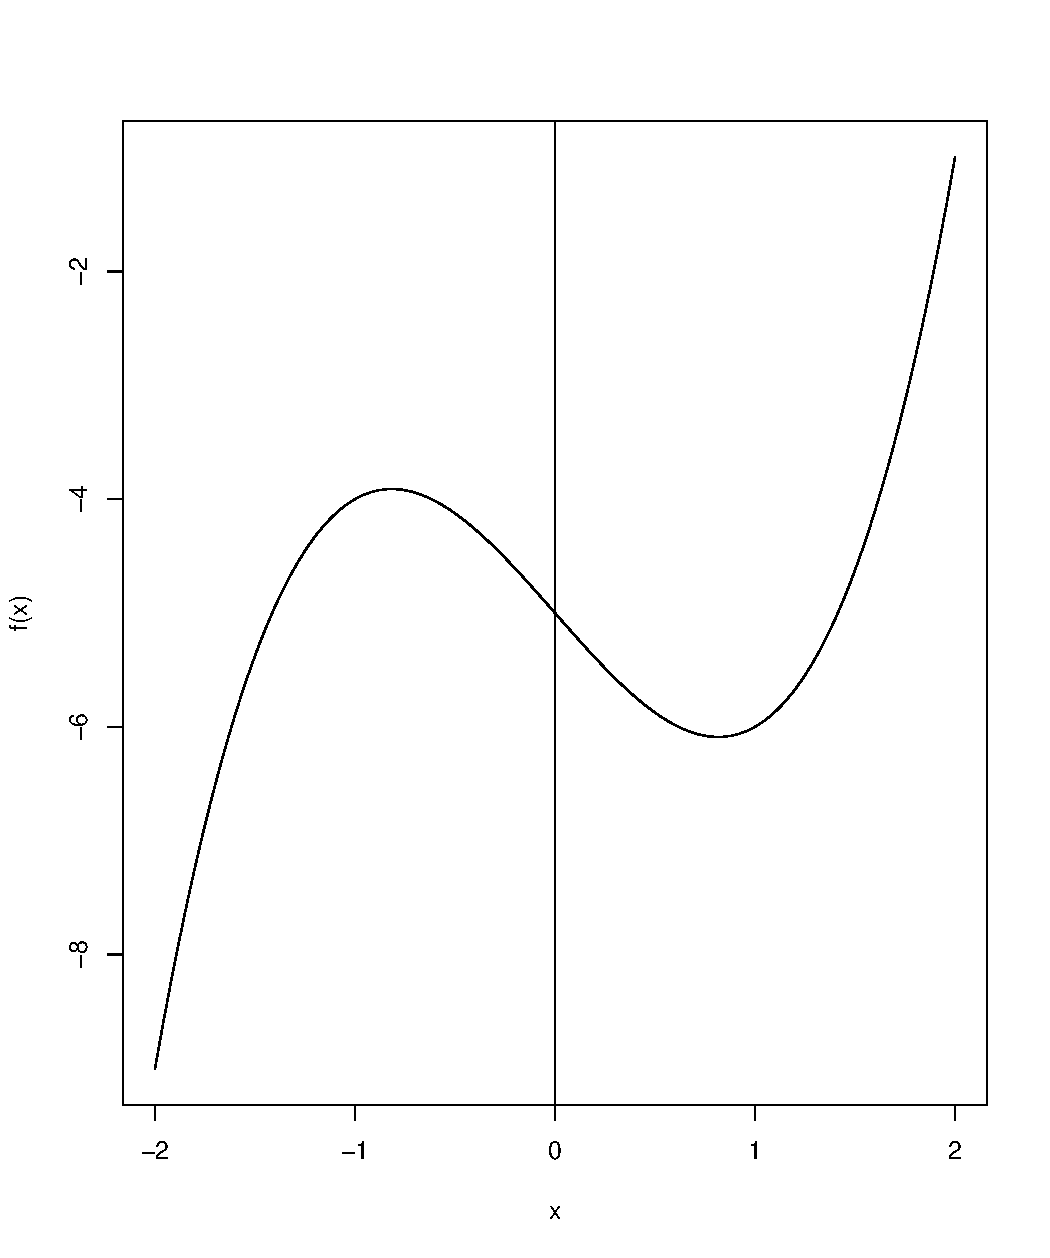
\includegraphics[scale=.8]{G3}
\caption{Grafica de la funcion 1}
\label{fig:G3}
\end{figure}

\begin{tabular}{| c | c | c | c |}
\hline
a & b & m & ERROR \\ \hline
 2.0000000   &    3.5000000   &    3.5000000   &    0.7500000      \\
 2.0000000   &    2.7500000   &    2.7500000   &    0.3750000      \\
 2.0000000   &    2.3750000   &    2.3750000   &    0.1875000      \\
 2.0000000   &    2.1875000   &    2.1875000   &    0.0937500      \\
 2.0937500   &    2.1875000   &    2.0937500   &    0.0468750      \\
 2.0937500   &    2.1406250   &    2.1406250   &    0.0234375      \\
 2.0937500   &    2.1171875   &    2.1171875   &    0.0117188      \\
 2.0937500   &    2.1054688   &    2.1054688   &    0.0058594      \\
 2.0937500   &    2.0996094   &    2.0996094   &    0.0029297      \\
 2.0937500   &    2.0966797   &    2.0966797   &    0.0014648      \\
 2.0937500   &    2.0952148   &    2.0952148   &    0.0007324      \\
 2.0944824   &    2.0952148   &    2.0944824   &    0.0003662      \\
 2.0944824   &    2.0948486   &    2.0948486   &    0.0001831      \\
 2.0944824   &    2.0946655   &    2.0946655   &    0.0000916      \\
 2.0944824   &    2.0945740   &    2.0945740   &    0.0000458      \\
 2.0945282   &    2.0945740   &    2.0945282   &    0.0000229		\\
 2.0945511   &    2.0945740   &    2.0945511   &    0.0000114      \\
 2.0945511   &    2.0945625   &    2.0945625   &    0.0000057      \\
 2.0945511   &    2.0945568   &    2.0945568   &    0.0000029      \\
 2.0945511   &    2.0945539   &    2.0945539   &    0.0000014      \\
 2.0945511   &    2.0945525   &    2.0945525   &    0.0000007   \\  \hline
\end{tabular}

\bibliography{BIBLIO}
\bibliographystyle{plainnat}

\end{document}